
%% ------------- English version ---------------
\documentclass[english]{sbrt}
\usepackage[english]{babel}
\usepackage[utf8]{inputenc}
\usepackage{amsmath}
\usepackage[shortlabels]{enumitem}
\usepackage{tikz}
\usetikzlibrary{arrows.meta,positioning}
\newtheorem{theorem}{Theorem}
%% ---------------------------------------------

\begin{document}

\title{ET-291 SAR \\ 2º Lista de Exercícios}

\author{Victor Davi dos Santos Bastos e Gabriel Luiz Espindola Pedro
    %\thanks{Name1 Surname1, Department1, University1, City1-State1, e-mail: xxxxx@yyyyy.zzzzz.br; Name2 Surname2, Department2, University2, City2-state2, e-mail: xxxxx@yyyyy.zzzzz.br. This work was partially supported by XXXXXXX (XX/XXXXX-X).}%
}

\maketitle

% \markboth{XLI BRAZILIAN SYMPOSIUM ON TELECOMMUNICATIONS AND SIGNAL PROCESSING - SBrT 2023, OCTOBER 08--11, 2023, S\~{A}O JOSÉ DOS CAMPOS, SP}{}


% \begin{abstract}
% This document is an example of how to use the \LaTeX\ style sbrt.cls to prepare a paper for submission to SBrT~2023. The abstract must have at most 100 words.
% \end{abstract}
% \begin{keywords}
% Paper template, \LaTeX, SBrT~2023.
% \end{keywords}


\section{Exercício 1}

Reproduzir a janela de Kaiser para diferentes valores de $\beta$

\begin{figure}[htb]
    \centering
    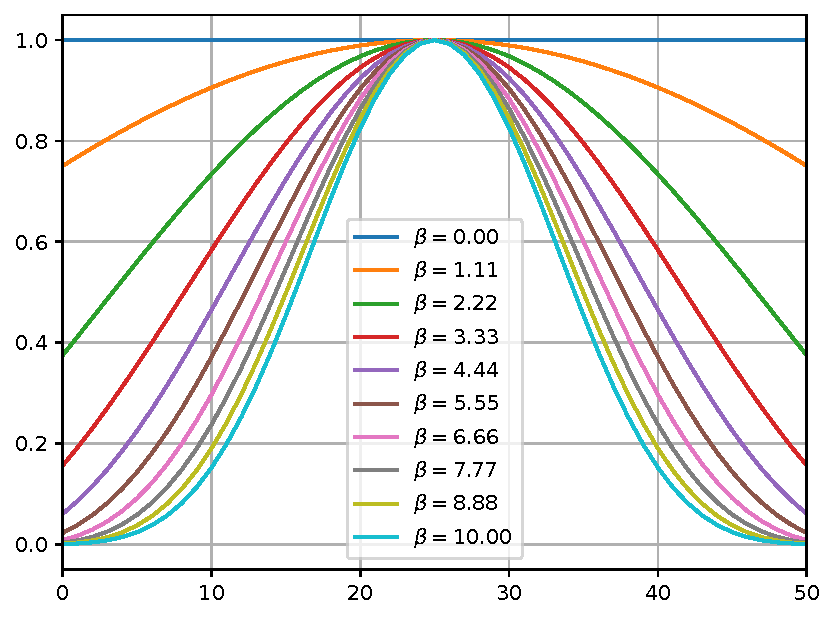
\includegraphics[width=0.95\linewidth]{kaiser_beta.pdf}
    \caption{Exercício 1}
    \label{fig:Exercício 1}
\end{figure}

\section{Exercício 2}

Simular um sinal amostrado. Criar uma função mais completa (com mais amostras) considerando a interpolação com diferentes kernels. Avalie os resultados obtidos. Avalie a precisão do interpolador.

\begin{figure}[htb]
    \centering
    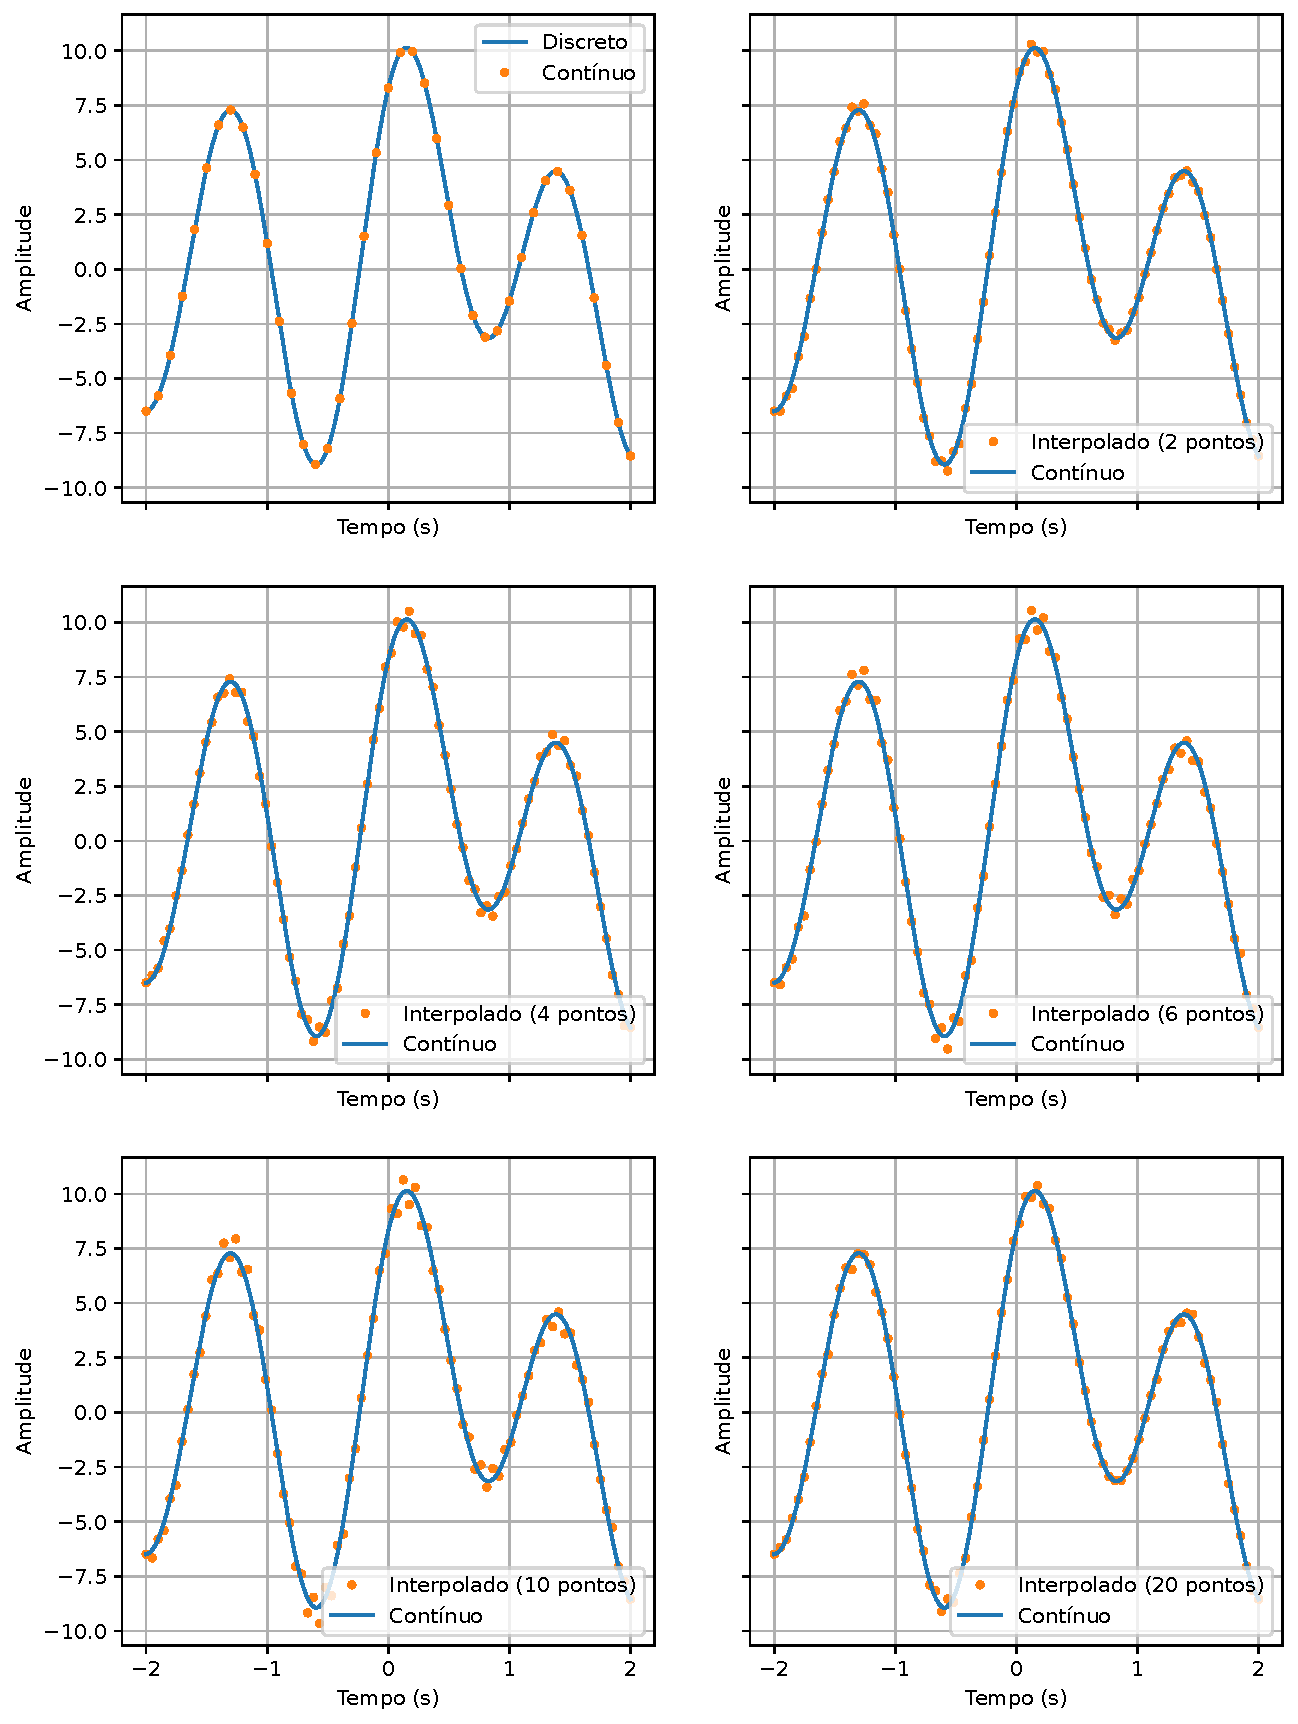
\includegraphics[width=0.95\linewidth]{interpolation.pdf}
    \caption{Exercício 2}
    \label{fig:Exercício 2}
\end{figure}

\section{Exercício 3}

Reproduzir (usando Matlab/Python) a figura do slide anterior.

\begin{figure}[htb]
    \centering
    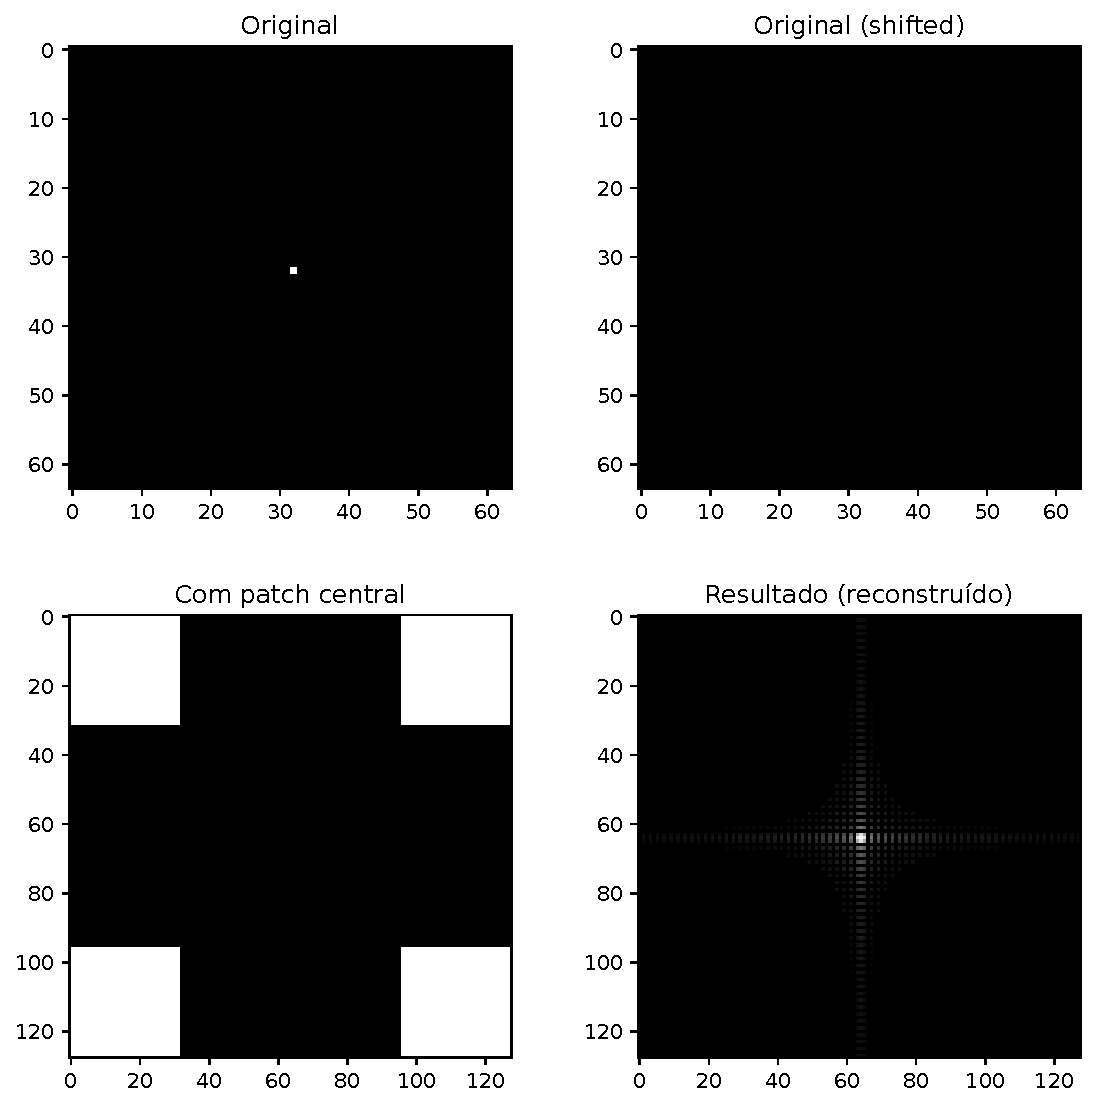
\includegraphics[width=0.95\linewidth]{point_target.pdf}
    \caption{Exercício 3}
    \label{fig:Exercício 3}
\end{figure}


\end{document}